% $Id: Grid_desc.tex,v 1.10 2007/05/17 22:16:57 cdeluca Exp $
%
% Earth System Modeling Framework
% Copyright 2002-2008, University Corporation for Atmospheric Research, 
% Massachusetts Institute of Technology, Geophysical Fluid Dynamics 
% Laboratory, University of Michigan, National Centers for Environmental 
% Prediction, Los Alamos National Laboratory, Argonne National Laboratory, 
% NASA Goddard Space Flight Center.
% Licensed under the University of Illinois-NCSA License.

The ESMF Grid class is used to describe the geometry and discretization
of a structured physical grid.  It also contains the description of the
grid's underlying topology and the decomposition of the physical grid
across the available computational resources.  The most frequent 
use of the Grid class is to describe physical grids in user
code so that sufficient information is available to perform ESMF
methods such as regridding. 

\begin{center}
\begin{tabular}{|p{6in}|}
\hline
\vspace{.01in}
{\bf Key Features} \\[.01in]
Representation of structured grids, including uniform and
rectilinear grids (e.g. lat-lon grids), curvilinear grids (e.g. displaced pole grids), 
and grids formed by connected logically rectangular regions (e.g. cubed
sphere grids).\\
Support for 2D, 3D, and higher dimension grids.\\ 
Distribution of grids across computational resources for parallel
operations -  users set which grid dimensions are distributed.\\
Options to define periodicity implicitly via standard shapes
(e.g. sphere, rectangle) or specify it explicitly.\\ 
Options for users to define grid coordinates themselves or call
prefabricated coordinate generation routines for standard grids.\\
Options for one-shot or incremental construction of grids.\\
Options for using a set of pre-defined stagger locations or for setting
custom stagger locations.\\[.03in] \hline
\end{tabular}
\end{center}

\subsubsection{Supported Grids}

The Grid class is based on the concepts described in {\it A Standard Descriptor 
of Grids Used in Earth System Models} \cite{BalajiGridSpec}.  In this document
Balaji introduces the {\bf mosaic} as a general construct useful for
describing a wide variety of Earth system
model grids.  A mosaic is composed of {\bf logically rectangular} grid {\bf tiles}
connected at their edges.  Mosaic grids includes simple, single tile grids as
a special case.

Grid tiles can have uniform, rectilinear, or curvilinear
coordinates.  The coordinates of {\bf uniform} grids are equally spaced along their
axes, and can be fully specified by the coordinates of the two opposing points
that define the grid's physical span.  The coordinates of {\bf rectilinear} grids
are unequally spaced along their axes, and can be fully specified by giving
the spacing of grid points along each axis.  The coordinates of {\bf curvilinear 
grids} must be specified by giving the explicit set of coordinates for each
grid point.  Curvilinear grids are often uniform or rectangular grids that 
have been warped; for example, to place a pole over a land mass so that it
does not affect the computations performed on an ocean model grid.  Any of
these logically rectangular grids can be combined through edge connections
to form a mosaic.  Figure \ref{fig:LogRectGrids} 
\begin{center}
\begin{figure}
\scalebox{0.9}{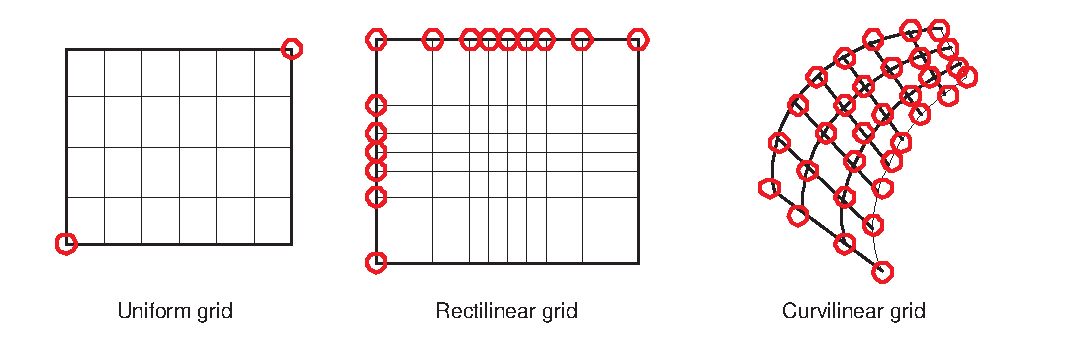
\includegraphics{LogRectGrids}}
\caption{Types of logically rectangular grid tiles.  Red circles show the
values needed to specify grid coordinates for each type.}
\label{fig:LogRectGrids}
\end{figure}
\end{center}

\subsubsection{Grid Classes in ESMF}

The ESMF Grid class is a representation of a mosaic grid.  Each ESMF
Grid is constructed of one or more Tiles. The DistGrid class enables
the user to define complex connections among Tiles such as those used in
cubed sphere grids.  A Tile will usually have some physical significance
(e.g. the region of the world covered by one face of a cubed sphere grid).  

The piece of a Tile which resides on one DE is
called a {\bf LocalTile}. For example, the six faces of a cubed sphere
Grid are each Tiles and each of the Tiles can be divided into many
LocalTiles by its distribution across DEs. 

\subsubsection{Options for Grid Creation} 

The Grid class is constructed using a layered approach to allow the 
users to select the level of control they want in interacting with
the Grid interface. At the highest level are the Grid Generation interfaces. 
These create a specific grid shape and fill in the appropriate coordinates. 
These will be implemented during a later phase of development. The
next level down are the specific shape grid creation interfaces (See Section~\textbf{Need Ref}). 
These allow the user to create a grid with a specific topology and 
distribution, but empty coordinate arrays. The lowest level are
the general grid creation interfaces (See Section~\textbf{Need Ref}). These allow the user
complete control over the description of their grids, but
make no assumptions about a specific topology or distribution. 

\subsubsection{Deferred Grid Creation}
 With a more complex interface such as that for Grid creation
for clarity's sake it is often useful to be able to proceed in stages
(e.g. setting various properties in understandable chunks). The 
Grid class provides the facility to do this using a set/commit paradigm.
This capability is also useful in distributing a grid object before
initialization or when multiple components contribute to the 
definition of a grid. Section~\ref{sec:usage:setcommit}
contains a description and example of this interface. 

\begin{tabular}{|p{2.6in}|p{1in}|p{1in}|p{1.4in}|}
\hline
\multicolumn{4}{|l|}{Options for Grid Creation} \\
\hline
Command sequence & Missing & Function & ESMF\_GRIDSTATUS\_ \\ 
\hline
ESMF\_GridCreateEmpty() 
& Topology information and coordinates, other options undefined
& Allocated placeholder that can be filled in
& NOT\_READY \\
\hline
ESMF\_GridCreate()\newline
{\bf or} \newline
ESMF\_GridCreateEmpty()\newline
ESMF\_GridSet()\newline
ESMF\_GridSet()\newline
...\newline
ESMF\_GridCommit(\newline
\indent ESMF\_GRIDSTATUS\_FIELD\_READY)\newline
{\bf or shortcut method, e.g.} \newline
ESMF\_GridCreateLatLonSphere()\newline
ESMF\_GridCreateLatLonRect()
& Coordinates
& Can be used as the basis for Field allocation
& FIELD\_READY\\
\hline
ESMF\_GridCreate()\newline
ESMF\_GridSetCoordFromArray()\newline
ESMF\_GridCommit(\newline
\indent ESMF\_GRIDSTATUS\_REGRID\_READY)\newline
{\bf or} \newline 
ESMF\_GridCreate()\newline
ESMF\_GridGetLocalTile(localTile)\newline
... user fills in localTile coordinate values
ESMF\_GridCommit(\newline
\indent ESMF\_GRIDSTATUS\_REGRID\_READY)\newline
{\bf or shortcut method, e.g.} \newline
ESMF\_GridCreateLatLonSphere()\newline
ESMF\_GridSetCoordLatLonSphere()\newline
ESMF\_GridCommit(\newline
ESMF\_GRIDSTATUS\_REGRID\_READY)
& Nothing; Grid is complete
& Can be used in regrid methods
& REGRID\_READY\\
\hline
\end{tabular}

\subsubsection{Factorized Coordinate Storage}

Often the coordinates for a grid do not vary across the entire
index space. For example, in a 2D rectilinear grid for a fixed y
index the y coordinate value will not change as x index changes,
and for a fixed x index the x coordinate value will not change as the
y index changes. In cases such as this the entire range of 
coordinates does not need to be stored, instead a reduced
(factorized) set of coordinate arrays can be stored which 
still describe the coordinates for the full grid, but at a large reduction in 
memory. Please see Section~\ref{sec:usage:coordstore} for
description and examples of the use of factorized coordinate
storage in ESMF Grids. 

\subsubsection{Staggering}

 A useful finite difference technique is to place different physical
quantities at different locations within a grid cell. This {\bf staggering}
of the physical variables on the mesh is introduced so that the difference
of a field is naturally defined at the location of another variable. When creating an 
ESMF Grid the user specifies which stagger locations the grid should 
contain (default is only the cell center).  Staggers can be set for up to the 
maximum grid dimension.  Later, when creating an  ESMF\_Field on the Grid the user
will specify upon which stagger location the Field and their data will reside.

There are predefined staggers and predefined stagger locations for ease of use,
however, the user can also specify their own if they need something different 
(see Section~\ref{ref:stagger} for a more in depth discussion of staggers).
 
For examples and a full description of the stagger interface 
please see Section~\ref{sec:usage:staggerloc}. 

To add:

{\bf Treatment of global and global data}{br}
 


